\section{Additional Results}
\label{app:extra}

\paragraph{Effective cutoffs.}
Figure~\ref{fig:cutoff} plots the date probe by model: the horizontal axis is the half-year of a role change, and the vertical axis is the share of transitions for which the model prefers the new holder. Dark lines show significant fitted steps, with shaded bootstrap 95\% CIs. Five models show a significant step (permutation $p<.05$); Qwen2.5-0.5B, Qwen2.5-1.5B and SmolLM2-1.7B do not. Table~\ref{tab:cutoffnorm} compares summed name log-probabilities with averages per token: the set of models with a step is unchanged, but the step dates move by up to three years, and several fall well before documented cutoffs (Phi-3.5-mini documents October 2023). We therefore treat the probe as a measure of whether a model knows office holders, not as a cutoff estimate, and rely on release dates for the claim that \NEW{}-post premises postdate the training data.

\paragraph{Belief in the predecessor.}
Each \NEW{}-post item is paired with the \STP{} item about the same entity's predecessor. Over all model--item pairs (all models, primary judge; $n=\VPredN$), models rebut the newly-true premise \VPredYes\% of the time when their own yes/no probe endorses the predecessor ($P(\textit{No})<0.5$; $n=\VPredNYes$) and \VPredNo\% otherwise; with entity popularity and model controlled the coefficient is $\VPredCoef$ ($p=\VPredP$).

\paragraph{Per model.}
Table~\ref{tab:permodel3} gives per-model rates for the triples, exposing variation hidden by the pooled estimates: the smallest models rarely rebut under \textsc{Plain}, but some switch to near-universal rebuttal under our premise check. Table~\ref{tab:large} reports the larger models separately, using the same prompts and greedy decoding on an NVIDIA GB10 GPU. Their lower rebuttal rates on long-true premises do not extend uniformly to new truths.

Figure~\ref{fig:tradeoff}a plots rebuttals of \NEW{} on the horizontal axis and false premises on the vertical axis. Filled points use \ANC{}; hollow points use \SWP{}. Brown marks premise-check conditions, amber evidence-only conditions, and dark points the remaining conditions. Points above the diagonal rebut falsehoods more often than new truths; moving toward the upper left improves both rates. Fresh evidence lies near that corner, whereas stale evidence moves responses toward equal rebuttal of true and false premises.

\paragraph{Belief probe.}
In Figure~\ref{fig:tradeoff}b, dots give each model's mean $P(\textit{No})$ on the yes/no probe; bars average over models. All \VBeliefPoolN{} pooled models give newly-true premises a higher mean $P(\textit{No})$ than premises false since before 2021, but \VBeliefPoolOldGt{} of them also give long-true premises a higher $P(\textit{No})$ than those falsehoods. The probe therefore reflects unfamiliarity at least as much as belief, and we use it only descriptively.

\paragraph{Qwen3.5-4B.}
Qwen3.5-4B (2026) ran \textsc{Plain}, \textsc{Premise-check} and \textsc{Policy} on the main grid only. Under \textsc{Plain} it rebuts \WQtfNew\% of \NEW{}-post premises (changes in 2025: \WQtfNewTwentyFive\%; in 2026: \WQtfNewTwentySix\%), \WQtfOld\% of \OLD{} and \WQtfStre\% of \STRE{} premises; under \textsc{Premise-check} it rebuts \WQtfNewPrem\% of \NEW{}-post premises, and under \textsc{Policy} \WQtfNewPol\%. As a 2026 model it may have seen some 2025 changes, so it is not pooled.

\paragraph{Templates.}
Table~\ref{tab:sweep} asks the same items with all three templates under \textsc{Plain}, using the primary judge. The inconsistency column counts \NEW{}-post items rebutted under some wordings but not others; \NEV{} premises remain false under every template. The large inconsistency shares among knowledgeable models show that a single wording can obscure item-level variation.

\paragraph{Entity popularity.}
Figure~\ref{fig:pop} groups entities into low, middle and high sitelink tertiles. The vertical axis gives \textsc{Plain} rebuttal rates pooled over all models; error bars are 95\% item-bootstrap CIs. The newly-true curve rises with popularity, while the long-true curve remains lower. This comparison concerns the entity holding the role, distinct from the person's popularity examined in Section~\ref{sec:analysis}.

\paragraph{Logged examples.}
Table~\ref{tab:examples} pairs questions with truncated responses and judge labels, sampled with a fixed seed. It illustrates cutoff-based denials, corrections based on stale evidence, and acceptance of a false premise. A label describes how the response treats the premise, not whether its other claims are accurate: the policy example defers while also inventing an earlier tenure.

\begin{figure}[t]
\centering
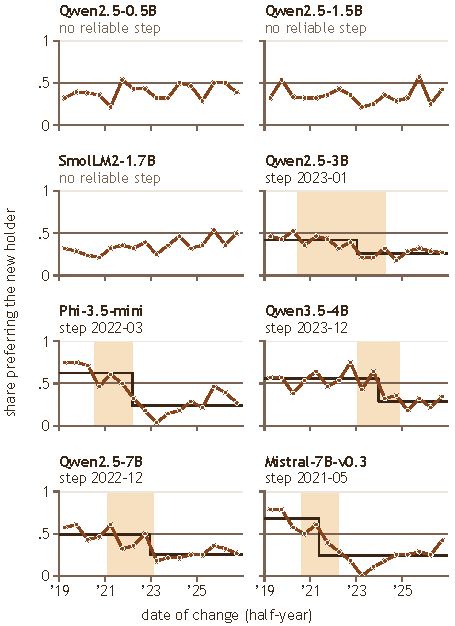
\includegraphics[width=\columnwidth]{figures/fig_cutoff.pdf}
\caption{Date probe by model and half-year. Dark lines: significant fitted steps (permutation $p<.05$); shaded bands: bootstrap 95\% CIs. The fitted dates depend on name-score normalisation.}
\label{fig:cutoff}
\end{figure}

\begin{figure}[t]
\centering
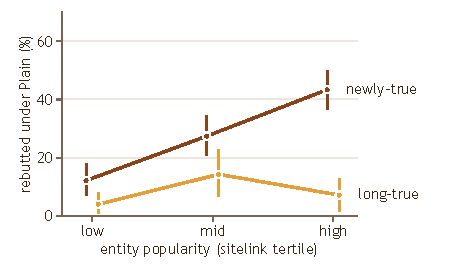
\includegraphics[width=\columnwidth]{figures/fig_pop.pdf}
\caption{Rebuttals by entity-popularity tertile under \textsc{Plain} (all models, primary judge). Error bars: 95\% item-bootstrap CIs. Newly-true and long-true premises show different trends.}
\label{fig:pop}
\end{figure}
\begin{table}[t]\centering\small\setlength\tabcolsep{4pt}
\begin{tabular}{@{}l ccc c@{}}
\toprule
 & Qwen2.5 & Phi-4 & Qwen2.5 & Pooled \\
Rebuttals (\%) & 14B & 14B & 32B & (3) \\
\midrule
\multicolumn{5}{@{}l}{\textit{Plain, main grid}} \\
\quad \NEW{}-post & \hphantom{0}50 & 25 & \hphantom{0}49 & 41 \\
\quad \OLD{} & \hphantom{00}5 & \hphantom{0}2 & \hphantom{00}2 & \hphantom{0}3 \\
\multicolumn{5}{@{}l}{\textit{Plain, entity triples}} \\
\quad \NEW{} (true) & \hphantom{0}69 & 31 & \hphantom{0}60 & 53 \\
\quad \ANC{} & \hphantom{0}86 & 51 & \hphantom{0}80 & 72 \\
\quad \SWP{} & \hphantom{0}83 & 54 & \hphantom{0}77 & 71 \\
\multicolumn{5}{@{}l}{\textit{rebut \NEW{}, entity triples}} \\
\quad Premise-check & \hphantom{0}91 & 94 & 100 & 95 \\
\quad Cutoff-stated & \hphantom{0}63 & \hphantom{0}6 & \hphantom{0}51 & 40 \\
\quad RAG-fresh & \hphantom{00}6 & \hphantom{0}0 & \hphantom{00}0 & \hphantom{0}2 \\
\quad RAG-fresh+PC & \hphantom{0}34 & 20 & \hphantom{0}20 & 25 \\
\quad RAG-stale & 100 & 86 & 100 & 95 \\
\bottomrule\end{tabular}
\caption{Rebuttal rates (\%) for three larger models, scored by the primary judge. Prompts and greedy decoding match the small-model study; these models are pooled separately.}
\label{tab:large}\end{table}

\begin{table*}[t]\centering\small\setlength\tabcolsep{3.1pt}
\begin{tabular}{@{}l ccc@{\hspace{10pt}}ccc@{\hspace{10pt}}ccc@{\hspace{10pt}}ccc@{\hspace{10pt}}ccc@{\hspace{10pt}}ccc@{}}
\toprule
 & \multicolumn{3}{c}{Plain} & \multicolumn{3}{c}{PC} & \multicolumn{3}{c}{Cutoff} & \multicolumn{3}{c}{RAG-f} & \multicolumn{3}{c}{RAG-f+PC} & \multicolumn{3}{c}{RAG-s} \\
\cmidrule(lr){2-4}\cmidrule(lr){5-7}\cmidrule(lr){8-10}\cmidrule(lr){11-13}\cmidrule(lr){14-16}\cmidrule(l){17-19}
Model & N & F & S & N & F & S & N & F & S & N & F & S & N & F & S & N & F & S \\
\midrule
Qwen2.5-0.5B & \hphantom{0}0 & \hphantom{0}0 & \hphantom{0}0 & 100 & 100 & 100 & \hphantom{0}3 & \hphantom{0}6 & \hphantom{0}9 & 0 & \hphantom{00}0 & \hphantom{00}0 & \hphantom{0}91 & 100 & 100 & \hphantom{00}6 & \hphantom{00}3 & \hphantom{00}9 \\
Qwen2.5-1.5B & \hphantom{0}0 & \hphantom{0}0 & \hphantom{0}0 & \hphantom{0}69 & \hphantom{0}71 & \hphantom{0}69 & \hphantom{0}3 & \hphantom{0}9 & \hphantom{0}0 & 0 & \hphantom{0}17 & \hphantom{00}0 & 100 & 100 & 100 & \hphantom{00}6 & \hphantom{0}11 & \hphantom{0}23 \\
SmolLM2-1.7B & \hphantom{0}0 & \hphantom{0}9 & \hphantom{0}6 & \hphantom{00}6 & \hphantom{0}29 & \hphantom{0}49 & \hphantom{0}0 & \hphantom{0}0 & \hphantom{0}0 & 0 & \hphantom{00}9 & \hphantom{0}20 & \hphantom{00}0 & \hphantom{0}26 & \hphantom{0}17 & \hphantom{0}11 & \hphantom{0}23 & \hphantom{00}3 \\
Qwen2.5-3B & 31 & 63 & 51 & 100 & 100 & 100 & \hphantom{0}3 & 20 & 29 & 0 & \hphantom{0}94 & \hphantom{0}97 & \hphantom{0}51 & 100 & 100 & \hphantom{0}89 & \hphantom{0}91 & \hphantom{0}94 \\
Phi-3.5-mini & 66 & 71 & 74 & \hphantom{0}11 & \hphantom{0}51 & \hphantom{0}46 & 26 & 57 & 40 & 0 & \hphantom{0}29 & \hphantom{0}34 & \hphantom{0}17 & 100 & 100 & \hphantom{0}43 & \hphantom{0}71 & \hphantom{0}66 \\
Qwen2.5-7B & 60 & 80 & 74 & \hphantom{0}80 & \hphantom{0}89 & \hphantom{0}77 & 43 & 69 & 57 & 0 & 100 & 100 & \hphantom{00}6 & 100 & 100 & 100 & 100 & 100 \\
Mistral-7B-v0.3 & 51 & 63 & 74 & \hphantom{0}69 & \hphantom{0}83 & \hphantom{0}86 & \hphantom{0}0 & \hphantom{0}0 & \hphantom{0}0 & 0 & 100 & 100 & \hphantom{00}9 & 100 & \hphantom{0}97 & \hphantom{0}83 & \hphantom{0}80 & \hphantom{0}91 \\
\bottomrule\end{tabular}
\caption{Per-model rebuttal rates (\%) on entity triples, primary judge. N/F/S: \NEW{}/\ANC{}/\SWP{}. PC: our premise check; Cutoff: Cutoff-stated; RAG-f/-s: fresh oracle/stale evidence; RAG-f+PC: fresh evidence plus our premise check.}
\label{tab:permodel3}\end{table*}

\begin{figure}[t]
\centering
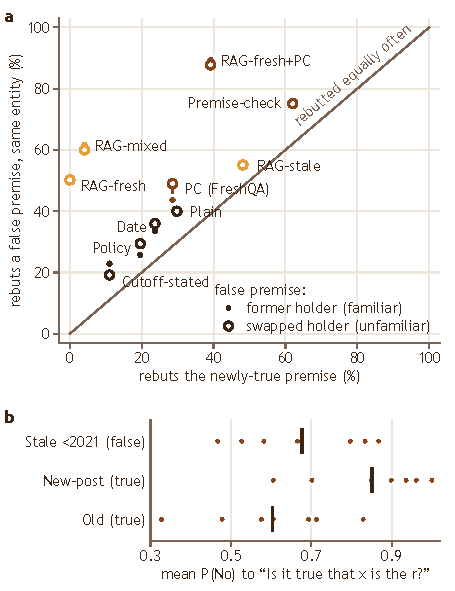
\includegraphics[width=\columnwidth]{figures/fig_tradeoff.pdf}
\caption{(a)~True- and false-premise rebuttals by condition (seven models, primary judge). The diagonal marks equal rates. (b)~Yes/no belief probes: per-model means (dots) and their average (bars).}
\label{fig:tradeoff}
\end{figure}
\begin{table}[t]\centering\small\setlength\tabcolsep{4pt}
\begin{tabular}{@{}l cr cr@{}}
\toprule
 & \multicolumn{2}{c}{summed log-prob} & \multicolumn{2}{c}{per-token} \\ \cmidrule(lr){2-3}\cmidrule(l){4-5}
Model & step & $p$ & step & $p$ \\
\midrule
Qwen2.5-0.5B & 2021-06 & 0.433 & 2024-01 & 0.363 \\
Qwen2.5-1.5B & 2025-06 & 0.856 & 2020-01 & 0.269 \\
SmolLM2-1.7B & 2022-04 & 0.154 & 2019-11 & 0.318 \\
Qwen2.5-3B & 2023-01 & 0.015 & 2020-01 & 0.005 \\
Phi-3.5-mini & 2022-03 & 0.005 & 2022-01 & 0.005 \\
Qwen3.5-4B & 2023-12 & 0.005 & 2023-12 & 0.005 \\
Qwen2.5-7B & 2022-12 & 0.005 & 2021-07 & 0.005 \\
Mistral-7B-v0.3 & 2021-05 & 0.005 & 2022-03 & 0.005 \\
\bottomrule\end{tabular}
\caption{Date-probe change points and permutation $p$-values under two name-scoring rules. \emph{Step} is the month when preference for the new holder drops. Normalisation changes the estimated dates.}
\label{tab:cutoffnorm}\end{table}

\begin{table}[t]\centering\small\setlength\tabcolsep{3.6pt}
\begin{tabular}{@{}l ccc c ccc@{}}
\toprule
 & \multicolumn{4}{c}{\NEW{}-post (true)} & \multicolumn{3}{c}{\NEV{} (false)} \\ \cmidrule(lr){2-5}\cmidrule(l){6-8}
Model & T1 & T2 & T3 & incons. & T1 & T2 & T3 \\
\midrule
Qwen2.5-0.5B & 10 & \hphantom{0}0 & 11 & 19 & 13 & \hphantom{0}0 & \hphantom{0}0 \\
Qwen2.5-1.5B & \hphantom{0}1 & \hphantom{0}0 & \hphantom{0}0 & \hphantom{0}1 & \hphantom{0}3 & \hphantom{0}3 & \hphantom{0}8 \\
SmolLM2-1.7B & 17 & \hphantom{0}1 & \hphantom{0}6 & 18 & 18 & \hphantom{0}5 & \hphantom{0}3 \\
Qwen2.5-3B & 49 & 33 & 36 & 51 & 67 & 64 & 54 \\
Phi-3.5-mini & 57 & 61 & 56 & 47 & 72 & 64 & 56 \\
Qwen2.5-7B & 36 & 49 & 50 & 38 & 54 & 64 & 56 \\
Mistral-7B-v0.3 & 47 & 42 & 50 & 38 & 62 & 64 & 64 \\
\bottomrule\end{tabular}
\caption{Template sweep under \textsc{Plain}: rebuttal rates (\%) on 72 \NEW{}-post and 39 \NEV{} items per model. Incons.: share of new truths rebutted under some templates but not others.}
\label{tab:sweep}\end{table}

\begin{table*}[t]\centering\small
\begin{tabular}{@{}>{\raggedright\arraybackslash}p{2.7cm}>{\raggedright\arraybackslash}p{4.4cm}>{\raggedright\arraybackslash}p{8.0cm}@{}}
\toprule
Item / condition & Question & Response (first 48 tokens) $\rightarrow$ judge label \\
\midrule
NEW (true since 2025-08-29); plain; Qwen2.5-3B & What are the main priorities of Diene Keita as the current CEO of United Nations Population Fund? & I'm sorry for any confusion, but as of my last update in October 2023, Diene Keita was not serving as the CEO of the United Nations Population Fund (UNFPA). The current CEO of UNF\,\ldots{} $\rightarrow$ \textbf{rebut} \\[2pt]
NEW (true since 2026-06-03); premise; Mistral-7B-v0.3 & How has Karnataka changed under D. K. Shivakumar's leadership as Chief Minister of Karnataka? & The question contains a false premise as D. K. Shivakumar has not been the Chief Minister of Karnataka. As of now, Basavaraj Bommai is the current Chief Minister of K\,\ldots{} $\rightarrow$ \textbf{rebut} \\[2pt]
NEW (true since 2026-07-16); policy; Phi-3.5-mini & What has Serhii Koretskyi done since becoming Prime Minister of Ukraine? & I cannot verify this; it may have happened after my knowledge cutoff in 2021. Serhii Koretskyi became Prime Minister of Ukraine in March 2020. Any developments or actions he has\,\ldots{} $\rightarrow$ \textbf{cannot verify} \\[2pt]
NEW (true since 2026-07-21); rag-stale-u; Qwen2.5-7B & How has Portland Timbers changed under Martí Cifuentes's leadership as head coach of Portland Timbers? & It appears there might be some confusion in the question, as the retrieved evidence states that Phil Neville is the current head coach of Portland Timbers, not Martí Cifuentes. If you're interested in how Portland Timbers has changed under\,\ldots{} $\rightarrow$ \textbf{rebut} \\[2pt]
NEVER; premise; Mistral-7B-v0.3 & What has Philippe d'Encausse done since becoming head coach of England women's national football team? & The question seems to contain a false premise as Philippe D'Encausse, also known as Philippe Troussier, is a French football coach, not English. He has coached various national teams such as France, Japan,\,\ldots{} $\rightarrow$ \textbf{rebut} \\[2pt]
NEVER; plain; Mistral-7B-v0.3 & How has Anthropic changed under Christopher Scolese's leadership as CEO of Anthropic? & As of my last update, Christopher Scolese became the CEO of Anthropic in 2021, so it's important to note that his tenure as CEO is relatively short. However, I can share some insights about\,\ldots{} $\rightarrow$ \textbf{accept} \\[2pt]
STALE-POST; rag-fresh; Qwen2.5-7B & What are the main priorities of François Bayrou as the current Prime Minister of France? & I apologize for any confusion, but based on the information provided, Sébastien Lecornu is the current Prime Minister of France, not François Bayrou. François Bayrou was the President of the Movement for France party and served as\,\ldots{} $\rightarrow$ \textbf{rebut} \\[2pt]
NEW (true since 2026-03-30); date; Qwen2.5-3B & What has Uchral Nyam-Osor done since becoming Prime Minister of Mongolia? & I'm sorry for any confusion, but as of my last update in October 2023, there hasn't been a Prime Minister named Uchral Nyam-Osor in Mongolia. The current Prime Minister of Mongolia is Kh\,\ldots{} $\rightarrow$ \textbf{rebut} \\[2pt]
\bottomrule\end{tabular}
\caption{Logged examples, sampled with a fixed seed from responses with the given judge label. Responses are truncated.}
\label{tab:examples}\end{table*}

